\documentclass[12pt]{report}
\usepackage[utf8]{inputenc}
\usepackage{graphicx}
\usepackage{amsmath}



\title{Communications requirements in delivery of vaccines by drones in covid-19 situation}
\author{Ivan Riolo }
\date{July 2021}

\begin{document}
\maketitle
\tableofcontents

\chapter{Overall idea}

In the field of health and logistic the delivery of medicines in remote and difficult to reach areas is one of the possible needs that can be solved using an IoT sensor system. In particular it's possible to use a type of UAV as vector to delivery medicines, like the 'quadcopters' drones that are the less expensive UAV. In recent times, the use of unmanned aerial vehicles such as drones is increasingly considered.
With particular attention to the current situation due to covid-19, a solution to this problem becomes even more relevant.
For example, it becomes very easy to deliver medicines faster in rural and poorly connected environments. Further benefit is the type of contactless delivery for example in a red zone. This type of logistic transport is addicted to the delivery of vaccines. More specifically this transport is suitable for the last part of the total journey, i.e. from the local center of a region to the surrounding areas. Therefore, it is not intended for the transport beyond about hundreds of kilometers where the main carrier becomes the aircraft. The use of systems of this type gives the possibility to monitor the temperature of vaccines and at the same time the position of them 
through specific sensors placed on the drones. Furthermore, considering the temperature limit to which vaccines must be subjected, each drone must be equipped with a thermal container. 
A possible way to satisfy this need is the creation of a wide area network in particular a low power wide area network that allows drones to communicate the information. One of the standards that meet the requirements of this scenario is LoRaWAN, considering the distances involved. 
A practical experiment with the same goal was announced in recent months by the American drone company Dragonfly. They have already successfully completed the transport of generic drugs via drones.

\begin{figure}[h!]
    \centering
    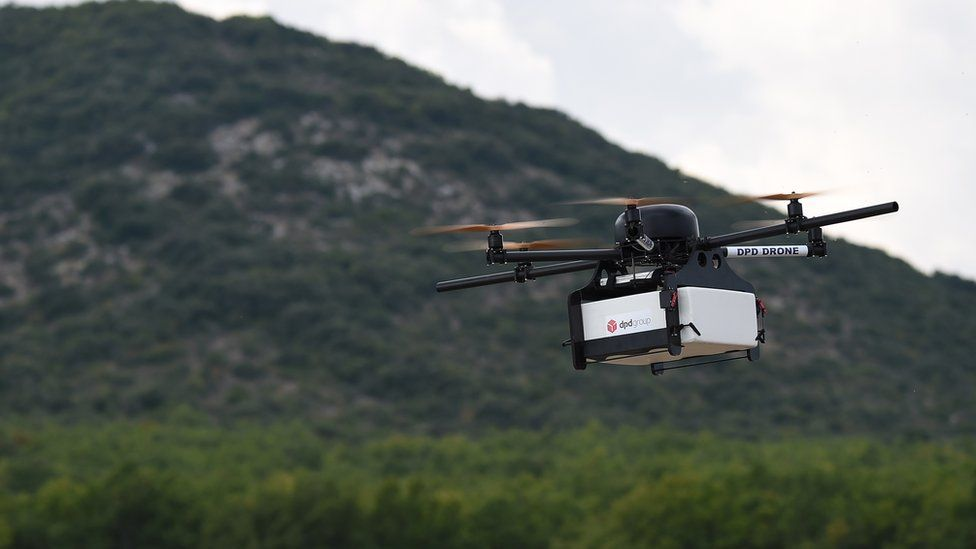
\includegraphics[width=14cm]{Pictures/Drone delivery.jpg}
    \caption{Vaccines delivery trial with a drone}
\end{figure}


\chapter{Communication requirements}

The two most important communication requirements in a scenario like the previous one are the
long range communication and the low power consumption communication. The first requirement is 
due to the fact that the drones must deliver the vaccines in a remote or difficult to reach 
area, so they have to communicate their data at distances of several kilometers. For the second
requirement, it must be considered that drones cannot be equipped with a heavy battery. 
Furthermore the radio transceiver is the part that requires the greatest energy consumption, 
without considering the energy required for flight. So, a low energy consumption mechanism 
must be chosen for the transmission of data. The above assumption leads to find a solution in 
the low power wide area network. In case of only monitor data the latency of transmission is not a very
critical parameter, so data can be received in semi real time. In case of critical situations, low latency is required to receive the parameters. The data are 
the following:
the temperature measured in the refrigerated box carried by the drone, and
the position measured by a gps receiver placed on the drone. It is possible to estimate the size of the payload to be inserted in each frame as follows. There are 3 floating values for latitude, longitude and height, each one is 32 bits long and in total a space of 12 bytes is required for these. While as regards the temperature it is possible to use also a decimal value, that is 32 bits long. In total, the payload will have a weight of 16 bytes, and considering the total frame it will be about 34 bytes long. An example of frame format is shown in the next figure where N = 16 bytes and M = 24 bytes. A compression algorithm can be used to reduce the weight of the data.

\begin{figure}[h!]
    \centering
    \includegraphics[width=14cm]{Pictures/Lora Packet.png}
    \caption{LoRa frame format}
\end{figure}
\newpage
Considering the energy saving as more important aspect, it is possible to accept 
a delay of a few seconds (2-3 s) in the transmission. For what concern data rate requirement, 
those meet perfectly the typical specification of LPWANs, maximum of 50 kbps in los and no 
interference condition, or a low data rate of 250 bps in high interference condition, can be enough. The 
link analyzed so far is the UAV-Gateway one. The second communication link inside this scenario is the Gateway-Network server, for
which there is no limitation of low energy as the gateway is usually a ground station connected
to electricity. The requirements for this link are defined by the type of architecture chosen 
considering the environment and the availability of 4G cellular network or wired ethernet 
network.


\chapter{Proposed architecture}

The architecture suitable for this scenario is the typical one of LPWANs proposed 
in the LoRaWAN protocol. In this environment is possible to identify the UAVs as end-nodes, 
while the gateways, are the sink nodes. For the choice of 
the type of connection between the Gateways and the Network server the following 
considerations must be made. These links can be done with a 4G connection using the cellular 
network or an Ethernet connection using a wired solution. Considering the environment in 
which the drones must operate, it is rural and difficult to reach area, so the deployment and 
installation of a wired network is very expensive and it may not be present. Considering that even
if there are cellular base stations (3G/4G cellular network), in this environment may not
guarantee a full coverage. 
Long-range communication in this case is an advantage, because is possible to choose as locations of gateways the positions
where cellular coverage is ensured. LoRa gateways antennas, thanks to their small size, are  
easy to deploy also in this environment. 
Therefore, in absence of a wired network, long-range communication between UAVs and 
gateways allows a simple deployment of ground stations where 3G/4G coverage is guarantee. All the intelligence is placed into the network server, responsible for confirming messages, avoiding duplicates, managing radio communication and security. At least one application server is connected to the server for example the one that is responsible of collecting and displaying data. 
Since there is no association between the mobile nodes and the gateways, an handover function is not necessary, the drones transmit their data in broadcast and the server selects the best quality ones. For this reason GPS sensor is necessary, tracking by exploiting the network with trilateration technique absorb more energy.

\begin{figure}[h!]
    \centering
    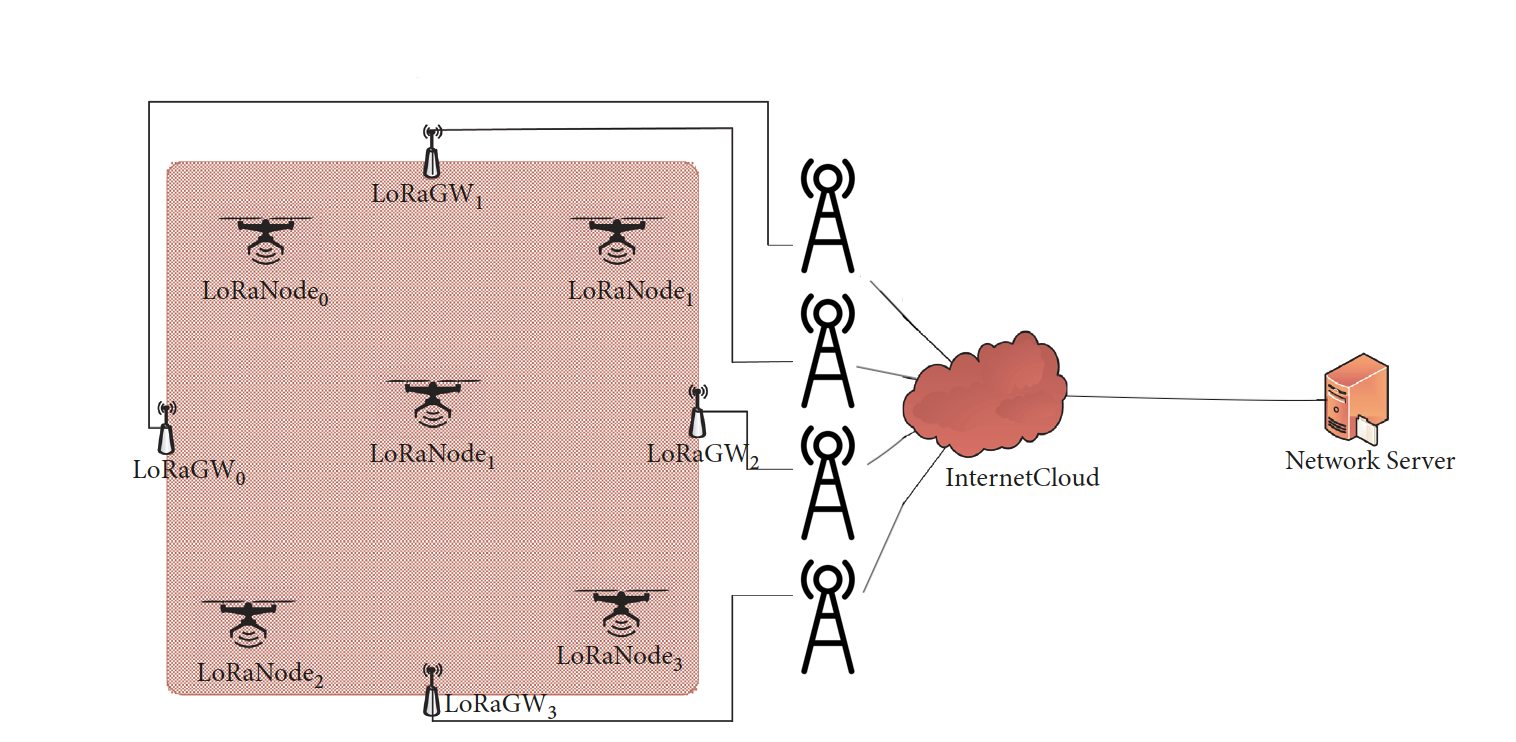
\includegraphics[width=14cm]{Pictures/High level arch.png}
    \caption{High level architecture}
\end{figure}

In the previous picture an example of chosen architecture is shown. The LoRaGWs are connected to the cellular base stations (3G or 4G) through which they reach internet and the server. In the rare case there is the availability of ethernet network it is also possible to use it.

\chapter{Chosen technologies}

Starting from the communication between the drones and the gateways, is possible to use the type B LoRaWAN end-node devices, because they can work also in the mode A that is the most energy saving mode. In fact, type A devices guarantees maximum energy savings in case there isn't need to download data at drones. Indeed, the most important data flow is from source nodes to the server network (uplink direction). In the EU the set of frequencies established for transmission in LPWANs is in the ISM band. 
Unfortunately there are severe limits to the duty cycle in this range, it must be equal to 1\%. This limit is used to ensure adequate usability to all possible users and to avoid possible interference, also considering that this portion of the band is unlicensed. So, after one frame transmission is necessary to wait 100-times its ToA. This limitation cause delay in transmission. A possible way to reduce this limit is to split a band in multiple sub-bands, in this way it possible to maintain a delay of few seconds between each transmission.  The modulation used for the transmission can be the proprietary chirped spread spectrum of LoRa or the traditional type of modulation like the FSK. The advantages of using the chirped spread spectrum one are the following. According to the channel condition by increasing the spreading factor (SF) it's possible to reduce data rate and avoid strong interference (i.e. SF12, 250 bps). While with decreasing the SF it's possible to increase data rate in low interference conditions (i.e. SF7, 11 kbps). Considering that in rural area the interference are very few its also possible to use a kind of modulation like the FSK one that allows to increase data rate at 50 kbps. The best choice is to use the chirped spread spectrum solution with an adaptive negotiation of SFs during the first connection to make the system more robust against interference. Other important benefit of this choice is the resistance to the doppler effect, considering that drones can achieve velocities of tens of km/h. In fact, thanks to the linearity of chirped signals the temporal offset are linearly related to the frequency offset, so it's easily eliminated in the decoder.

\begin{figure}[h!]
    \centering
    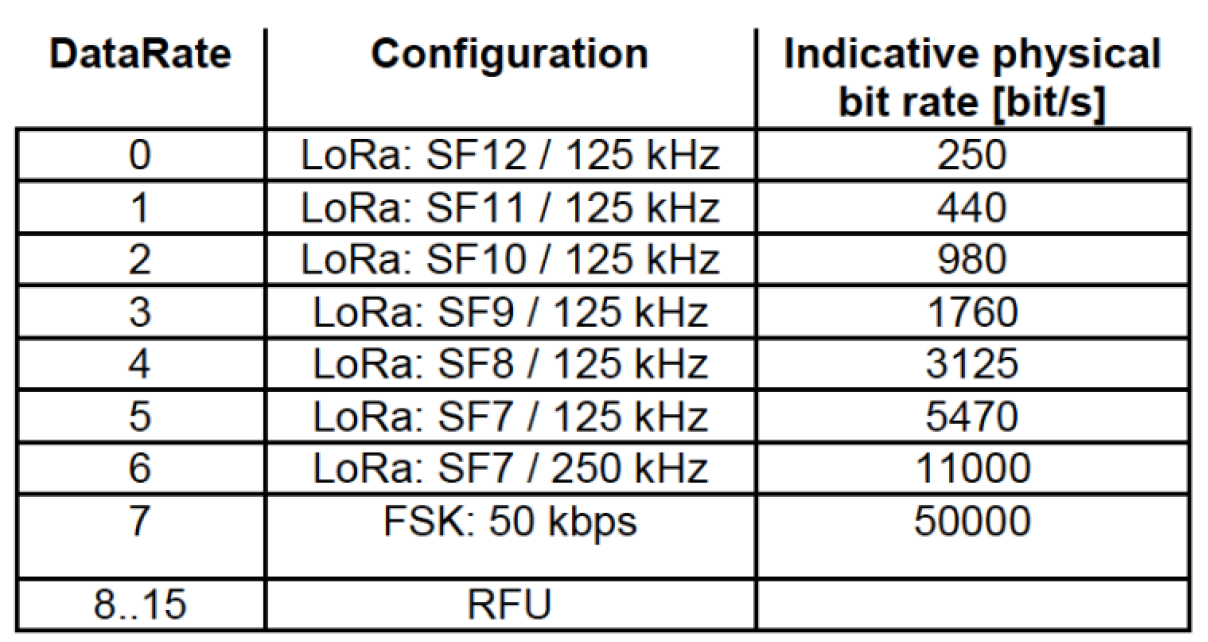
\includegraphics[width=10cm]{Pictures/SF data rates.png}
    \caption{SFs data rates table}
\end{figure}


An example of typical communication between the end node and the server is shown in the next figure. The LoRa mode A communication mode is preferred in not critical situation to monitor temperature and position at fixed intervals. The two DL windows is used only to confirm the messages of end devices. This saves a lot of energy.

\begin{figure}[h!]
    \centering
    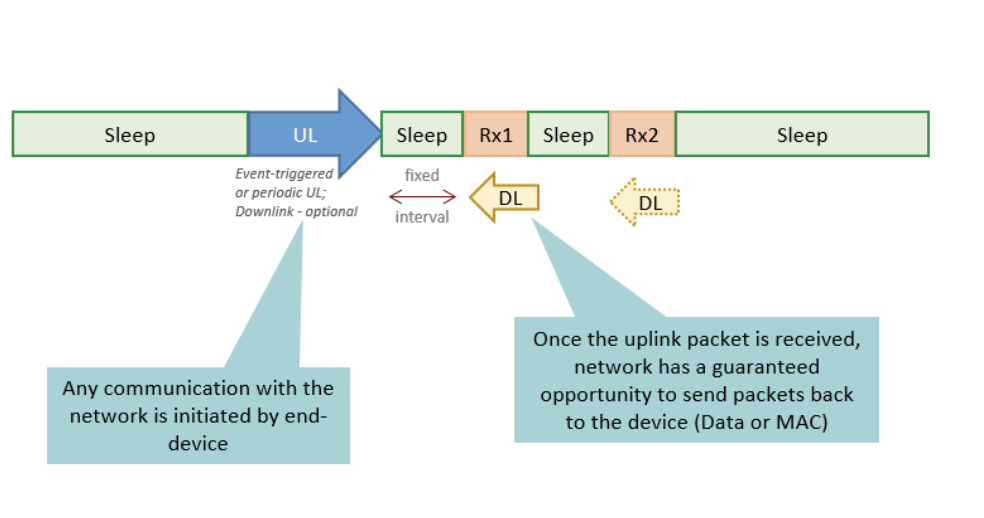
\includegraphics[width=10cm]{Pictures/Class A devices .png}
    \caption{Example of a normal exchange of control messages}
\end{figure}


While in a critical situation when something does not work correctly an alarm is activated, the LoRa mode B of communication is performed. As can be seen in the following figure, this mode determines an higher energy consumption by activating a beaconing function. In this way the end device is synchronized with the gateway and exchange messages in real time. This occurs only when, for example, the temperature of the vaccines falls below a certain threshold and allows for temperature and position tracking in low latency conditions.

\begin{figure}[h!]
    \centering
    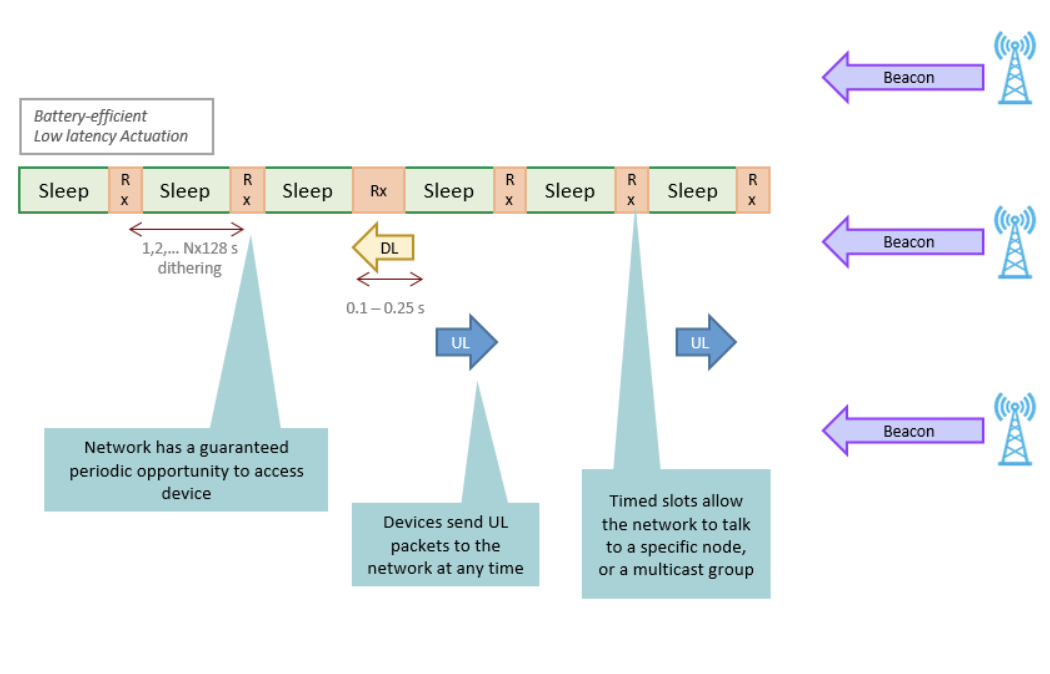
\includegraphics[width=10cm]{Pictures/Class B devices.png}
    \caption{Example of critical exchange of alarm messages}
\end{figure}


For what concern the server application technologies is possible to implement the so called TICK stack. With the use of these tools is possible to better collect, store, visualize and analyze time series data coming from the drones. The tools that performs these tasks are Telegraf, InfluxDB, Cronograf and Kapacitor.





\end{document}
